\documentclass{article}
 
\title{Make Your Own Lithium Power Banks}
\author{Demand for Energy Equality}
%inherited code
\usepackage{amsmath,amsthm,amssymb,epsfig}
\usepackage{hyperref}

% imports for images
\usepackage{caption}
% \usepackage[demo]{graphicx}
\usepackage{graphicx}
% \usepackage{float}

% import for resuming enumerated list
\usepackage{enumitem}

% code to remove numbering but keep the contents page filled
\setcounter{secnumdepth}{0}

\theoremstyle{definition}
\newtheorem{thm}{Theorem}[section]
\newtheorem{lem}[thm]{Lemma}
\newtheorem{prop}[thm]{Proposition}
\newtheorem{cor}[thm]{Corollary}
\newenvironment{pf}{{\noindent\sc Proof. }}{\qed}

\theoremstyle{definition}
\newtheorem*{defn}{Definition}
\newtheorem*{exmp}{Example}
\newtheorem*{prob}{Problem}
\newtheorem*{info}{Information}
\newtheorem*{warn}{Warning}
\newtheorem*{quest}{Question}
\newtheorem*{blockq}{Block Quote}
\newtheorem*{strong}{Strong}
\newtheorem*{code}{Code}
\newtheorem*{coderesult}{Code Result}

\theoremstyle{remark}
\newtheorem*{rem}{Remark}
\newtheorem*{note}{Note}
\newtheorem*{exer}{Exercise}

\setlength{\oddsidemargin}{0.25 in}
\setlength{\evensidemargin}{-0.25 in}
\setlength{\topmargin}{-0.6 in}
\setlength{\textwidth}{6.5 in}
\setlength{\textheight}{8.5 in}
\setlength{\headsep}{0.75 in}
\setlength{\parindent}{0 in}
\setlength{\parskip}{0.1 in}

%%%%%%%
% Some commonly used notation
%%%%%%%

\def\R{{\mathbb R}}
\def\X{{\mathcal X}}
\def\Y{{\mathcal Y}}
\def\E{{\mathbb E}}
\def\sign{{\rm sign}}

% END inherited code

\begin{document}
 
\maketitle{}

\begin{center}
  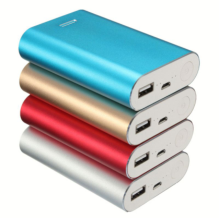
\includegraphics[]{Images/image_0_1_(power_banks).png}
\end{center}

\vfill
  

\includegraphics[]{Images/image_0_2_(license).png} \newline
This guide is provided under a \href{https://creativecommons.org/licenses/by-sa/4.0/legalcode}{Creative Commons BY-SA} license: \newline
Material may be freely shared and adapted under the following terms: You must give appropriate credit, provide a link to the license, and indicate if changes were made, and further distribution must be under the same license as the original.

\newpage

\tableofcontents

\newpage

\section{Introduction} % (fold)
\label{sec:introduction}

  \subsection{The Demand Energy Equality project} % (fold)
  \label{sub:the_demand_energy_equality_project}

    Demand Energy Equality (DEE) is a UK based community energy project that seeks to provide practical energy education using solar photovoltaics. We are a group working for systemic change in the way energy is produced, distributed, controlled, delivered and used. These aims are within the context of rising energy inequality (in the UK, at least), rising fuel bills, climate change and the increasing cost of fossil fuel extraction. See \href{https://www.demandenergyequality.org/about/}{our website} to find out more about the project.
    
    Through teaching hands-on energy skills we also aim to develop people’s relationship with energy, and enable them to understand it better; where it comes from, how it is used and how it relates to their needs. Ultimately we aim for this to change behaviour, leading to better use of energy and overall reduced demand. Reduced energy use is an unavoidable fact of the relatively near future – far better to prepare now than be surprised later on.
  
  % subsection the_demand_energy_equality_project (end)
  
  \subsection{Using this guide} % (fold)
  \label{sub:using_this_guide}

    This written guide explains the concepts and techniques involved in making small USB power packs using recovered lithium-ion battery cells. It assumes no prior knowledge of any kind relevant to completing a fully working project. The guide is designed to act as a learning aid for participants on the ‘Make Your Own Lithium Power Bank’ workshops run by Demand Energy Equality, and can be used alongside other DIY guides and resources provided by DEE. 
    
    The guide provides a summary of the basic concepts involved in energy systems, gives an explanation of what lithium cells are and how they can be used, and gives some tips on what you might need to know for larger DIY projects. Links to useful sources of further research are included at the end of the guide.
    
    This particular version reflects the most recent iteration of the process of building a power bank as practiced by DEE, but it is likely that it may evolve and expand over time. Because we occasionally review and update our content, the guide may not always be in line with the other DIY resources published by DEE, and may not exactly reflect the format of current workshops. Contact DEE if you need an update on any recent changes. 
    
    You will find the latest version of this guide available to download from the DEE website, as and when this guide is updated, alongside our \href{https://www.demandenergyequality.org/resources/}{other guides and resources}.
    
    For a chance to gain practical experience of the material covered in this guide, please take a look at the \href{https://www.demandenergyequality.org/our-workshops/}{workshops} offered on the DEE website.
    
    We encourage you to share the skills you learn with others through your own workshops, particularly if you are able to target and work with low-income communities. Please contact us for any support you feel you may need if you plan to do this.
  
  % subsection using_this_guide (end)
  
  \subsection{Disclaimer} % (fold)
  \label{sub:disclaimer}

    This guide is for general guidance only and whilst every effort is made to ensure that the information it contains is correct, it should not be relied upon as accurate. The information / advice contained within this guide is intended for use within the UK only and by persons of no less than 18 years of age. Use this guide at your own risk.
    
    DEE will not accept any liability for any loss, damage, injury or negligence, direct or indirect, from use of the information / advice contained within this guide.
  
  % subsection disclaimer (end)

  \newpage  

% section introduction (end)

\section{Basic concepts} % (fold)
\label{sec:basic_concepts}
  
  \subsection{Power consumption} % (fold)
  \label{sub:power_consumption}

    \textit{Power} is a measure of work done in any instant, measured in watts (W). You'll typically find a value of the number of watts an appliance needs to operate written on the outer case or on the adaptor that plugs into the wall socket. The power consumed when charging a smart phone, for example, is commonly around 6 watts. This is the measurement that tells you how much power you actually need to deliver for every moment that the appliance is in operation. To measure the overall work done by an appliance, you need to introduce time to the equation. The unit that is generally used to measure this in electrical systems is watt hours (Wh), which is a measurement of energy. Energy is directly related to power and time using the equation: 

    \begin{equation}
      \text{Energy} (Wh) = \text{Power} (W) \times \text{Time} (h)
    \end{equation}
    
    Understanding this relationship allows us to calculate the energy required to charge a smart phone for an hour: 6 Watts \(\times\) 1 hour = 6 Watt-hours.
  
  % subsection power_consumption (end)

  \subsection{Voltage} % (fold)
  \label{sub:voltage}

    \textit{Voltage} is the potential to do work. It is measured in volts (V). Imagining electricity like a flow of water turning a water wheel, the voltage is like the height of the flow of water flowing into the water wheel. If the voltage is too low the water will just flow underneath the water wheel and the water wheel won't turn. A higher voltage will turn the wheel effectively. A voltage too high could be damaging to the water wheel. In the same way a voltage too high for an appliance will damage the appliance.
  
  % subsection voltage (end)

  \subsection{Current} % (fold)
  \label{sub:current}

    \textit{Current} is the flow of electricity and is measured in amps (A). Using the same flow of water analogy current is the amount of water flowing. More flow allows the water wheel to turn faster, less flow makes it turn slower. For electrical systems, power is directly related to voltage and current using the equation:

    \begin{equation}
      \text{Power} (W) = \text{Voltage} (V) \times \text{Current} (A)
    \end{equation}

    Essentially what this means is that the amount of power available increases if either the volts or the amps increase, or of course if both increase. Similarly, the amount of power available decreases if either the volts or the amps decrease, or if both decrease.
  
  % subsection current (end)

  \subsection{Resistance} % (fold)
  \label{sub:resistance}

    \textit{Resistance} reduces the flow of electricity through a wire or component. It is a bit like forcing the water from our analogy to travel through a canyon filled with rapids. Relative to the same amount of water flowing through a smooth channel, the ability to deliver power at the other end will be reduced. All components and wires have an internal resistance that converts some of the electricity you are supplying into heat without doing any useful work. This is something we want to minimise in our systems. 
  
  % subsection resistance (end)

  \subsection{Series and parallel circuits} % (fold)
  \label{sub:series_and_parallel_circuits}

    Electrical circuits behave in different ways depending on how they are connected. There are two types of connections: 
      
      \begin{table}[!h!]
        \centering
        \begin{tabular}{|| c | c | c | c ||}
          \hline
          \multicolumn{2}{|c|}{Series Circuits}  & \multicolumn{2}{|c|}{Parallel Circuits}  \\
          \hline \hline
          Connect & $+ \rightarrow -$ & Connect & $+ \rightarrow +$ \\
          \hline
          Connect & $- \rightarrow +$ & Connect & $- \rightarrow -$ \\
          \hline
        \end{tabular}
        \label{table:two_types_of_connections}
      \end{table}

    Two components connected in series will each have their own voltage while the current will be the same through both. In terms of power sources (like panels and batteries) this means that the voltage will sum across components connected in series while the current will stay constant. 

    For simple electrical appliances connected in series, the total voltage from the power source will be shared between each component. For example, two identical 6V bulbs in series connected to a 12V battery will light up as expected, since each bulb will consume 12 \(\div\) 2 volts. The current through each bulb will be determined according to their power rating. Two 12V bulbs connected in series to a 12V battery will not light up properly - you may see a dim glow but as the voltage each bulb is using is only 6V this is not enough to properly light the bulbs.

    In parallel connections the voltage will be constant across the appliances and the current will be shared. In terms of power sources (like panels and batteries) this means that the voltage will be constant across the appliances and the current will sum. For power consumers (like appliances) connected in parallel, each appliance will have the full voltage available to it and each will share the total current drawn. So two 12V bulbs in parallel with a 12V battery will light up with a current draw equal to the sum of the two bulbs. Two 6V bulbs in parallel with a 12V battery will more than likely break as each will have 12V supplied to it, double what it requires. 

    \begin{figure}[!ht]
      \centering
      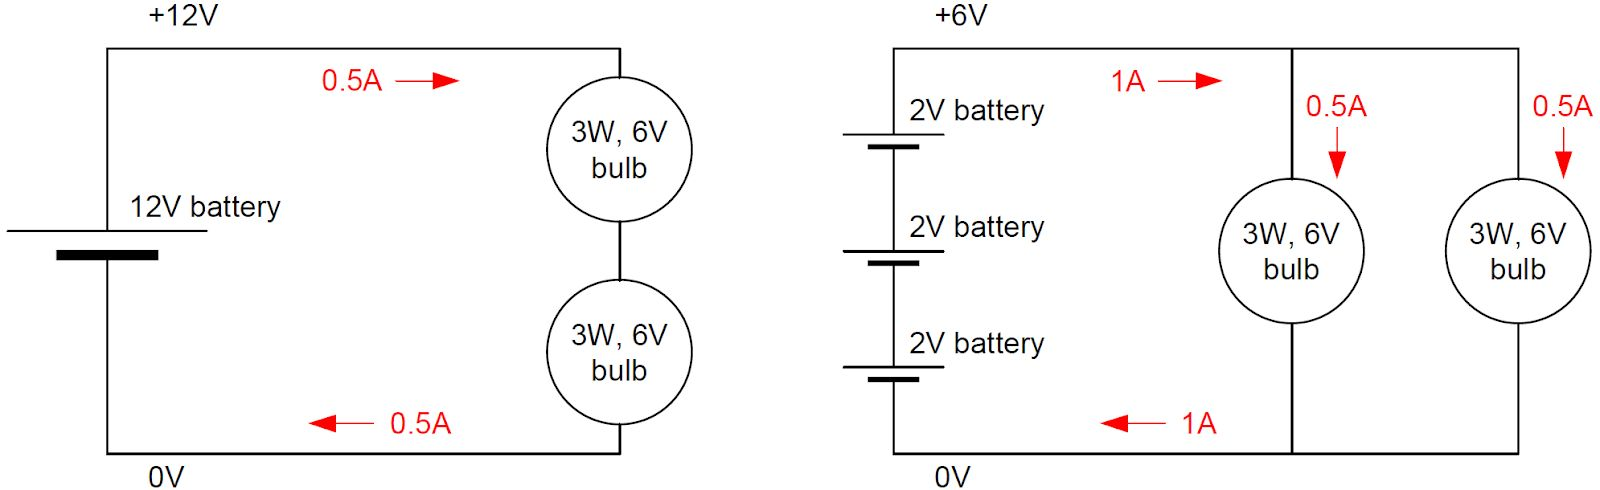
\includegraphics[width=0.75\paperwidth]{Images/image_2_1_(parallel_v_series_circuit).png}
        \caption*{\centering A 12V battery can power two 6V bulbs in series. Three 2V batteries in series can power two 6V bulbs in parallel.}
    \end{figure}

    Electrical appliances are generally designed to work with a specific power supply voltage, so be sure to only connect them in the right way. E.g. - if multiple 12V appliances are being used with a single 12V power supply, they should all be connected in parallel.
  
  % subsection series_and_parallel_circuits (end)

  \subsection{Battery capacity} % (fold)
  \label{sub:battery_capacity}

    To use a battery effectively, we need to know how much energy it can store. This is known as battery capacity, and is measured in Amp-hours (Ah). For small batteries you will usually see the capacity measured in milli-Amp-hours (mAh) - 1 Ah is 1000 mAh. This gives an indication of the battery’s capacity to deliver current over time. In theory a 6Ah battery could deliver 1A for 6 hours or 6A for 1 hours, although the more current is being drawn, the less capacity the battery will be able to deliver. 
  
    To calculate the overall energy that a battery can store, you multiply the capacity (in Ah) by the nominal voltage (in V) to give the energy in Watt-hours. Most lithium-ion cells have a nominal voltage of 3.7V, but not all, so make sure to check before using them. So a typical lithium cell with a capacity of 2000mAh (2Ah) and a nominal voltage of 3.7V will store 7.4Wh (2 \(\times\) 3.7) when fully charged.
  
  % subsection battery_capacity (end)

% section basic_concepts (end)

\section{Risks and dangers of lithium-ion batteries} % (fold)
\label{sec:risks_and_dangers_of_lithium_ion_batteries}

  Warning - proceed at your own risk. The electrolyte used in lithium-ion cells is extremely reactive, and extreme care must be taken when using them for DIY projects.

  When charging and discharging lithium-ion cells, be sure not to exceed their rated current. If in doubt, keep charging and discharging currents below 1 Amp per cell in parallel.

  Lithium-ion cells in storage should be kept cool, and ideally not fully charged

  \subsection{Minimising the risk of lithium-ion battery fires} % (fold)
  \label{sub:minimising_the_risk_of_lithium_ion_battery_fires}
  
    Most lithium-ion cells have low thermal stability, especially the types commonly found in phones and laptops. Thermal stability can be compromised further when fully charged (4.2V) or being charged at high currents (above 1C). Heat can be very damaging to the lifespan of a lithium-ion cell, and in the worst cases can cause thermal runaway, which leads to the electrolyte in the cell catching fire.

    Always protect lithium-ion cells against over voltage. Charging cells at voltages higher than 4.2V can lead to them catching fire.

    Working with unprotected lithium-ion cells carries a risk of creating accidental short circuits that can lead to cells catching fire. Always handle them with extreme care, especially when using metal tools close to them. Short-circuiting a cell can lead to it catching fire.

    Battery packs made from lithium-ion cells in series should only be charged with a suitable Battery Management System that monitors the voltage of each cell to ensure they remain balanced. If this is not done, cells can become unbalanced, leading to some cells being overcharged, that can result in the battery pack catching fire. 

    The internal structure of cells that have been overused or damaged can be affected to the point that they can form internal short circuits. Used cells should only be included in a battery if they have been thoroughly tested. Fusing individual cells in a lithium-ion battery pack can protect against internal short circuits, that would otherwise result in the cells catching fire.

  % subsection minimising_the_risk_of_lithium_ion_battery_fires (end)

% section risks_and_dangers_of_lithium_ion_batteries (end)

\section{What are lithium-ion battery cells?} % (fold)
\label{sec:what_are_lithium_ion_battery_cells}

  The use of lithium-ion batteries has been increasingly common since the late 1990s. For their size and weight they can store a relatively large amount of energy and are very reliable, but compared to other batteries such as lead-acid and nickel-metal-hydride they are expensive and more complicated to use. Their use has diversified and evolved over time resulting in a range of different lithium-ion chemistries that specialise in capacity, power and longevity. They can be found in mobile phones, laptops, rechargeable torches, cordless power tools, electric vehicles, and many other appliances. 

  Lithium-ion cells are commonly constructed of a carbon anode, a metal oxide cathode, and an electrolyte paste that contains lithium compounds. These are sandwiched together in very thin sheets with an insulating layer on the outside, that are either folded to create flat cells, or rolled to create cylindrical cells.

  The ‘swiss roll’ of a cylindrical cell is housed within a durable steel container that prevents the reactive elements inside the cell being exposed, and protects the cell from damage. The end caps on these cells include safety features such as vents that allow any gases that might build up inside the cell to escape. Flat cells are usually contained in a sealed pouch that can expand to contain any gases that might build up inside the cell. 

  \subsection{Comparing Lead-acid and Lithium batteries} % (fold)
  \label{sub:comparing_lead_acid_and_lithium_batteries}

    Lithium-ion (Li-ion) batteries have several advantages over conventional lead-acid batteries:

    Performance

      \begin{itemize}
        \item High energy density: more energy with less weight
        \item High charge currents (shortens the charge period)
        \item High discharge currents (enabling high power applications on a small battery bank)
        \item Long battery life (up to six times the battery life of a lead-acid battery)
        \item High energy charge cycle efficiency (a higher \% of the energy used to fully charge the battery can be delivered when discharged)
      \end{itemize}

    Life cycle cost

      \begin{itemize}
        \item Li-ion batteries are expensive when compared to lead-acid, but their superior reliability and efficiency can make them more cost-effective over their total lifespan, especially if being used in a situation where size and weight are critical factors. 
        \item Good quality lithium batteries are generally rated to be able to deliver many more charge-discharge cycles before losing significant capacity, compared to good quality deep cycle lead-acid batteries.
      \end{itemize}

  % subsection comparing_lead_acid_and_lithium_batteries (end)

  \subsection{Lithium-ion charging} % (fold)
  \label{sub:lithium_ion_charging}

    Battery chargers designed to be used with lead-acid batteries should never be used to charge lithium batteries. The final stage of charging a lead-acid battery is called the ‘float’ stage, where the charger will ‘trickle’ a small amount of current into the battery to compensate for self-discharge. With a lithium-ion battery, it’s very important that the voltage does not go above 4.2V, and the charge cycle should finish as soon as the battery is 100\% charged.

    \begin{figure}[!ht]
      \centering
      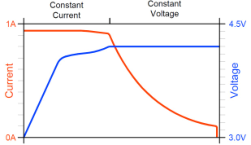
\includegraphics[]{Images/image_4_1_(charge_cycle).png}
      \caption*{\centering Lithium-ion charge cycle}
    \end{figure}

    The nominal voltage of a lithium-ion cell is 3.7V (or sometimes 3.6V), which represents the voltage when the cell is 50\% charged. A fully charged cell should have a voltage of 4.2V. A fully discharged cell should have a voltage of 3V.

  % subsection lithium_ion_charging (end)

  \subsection{Caring for lithium-ion batteries} % (fold)
  \label{sub:caring_for_lithium_ion_batteries}

    \textbf{Don’t overheat.} Lithium-ion cells can easily be damaged when subject to high temperatures - anything over 40 degrees should be avoided if possible. This can happen when the battery is being charged or discharged with high currents, which will generate additional heat.

    \textbf{Don’t leave fully charged.} For example, if using a laptop for an extended period of time, try not to leave the charger plugged in all the time. Some laptops have a battery saver setting, which will limit how much the battery is charged, so it only charges to 80\% of its full capacity. 

    \textbf{Don’t fully discharge.} The battery should be recharged when it reaches 10-20\% charge level. Expect to use 80\% of the overall battery capacity. 

    \textbf{Charge/discharge with low currents.} The C rating of a lithium-ion cell is the current needed to charge the cell in 1 hour, so a 2000mAh cell will have a C rating of 2 Amps. If you want cells to last as long as possible, it’s generally a good idea to avoid charging or discharging them above the C rating. Cells in parallel will share any load, so if high currents are required you can combine multiple cells together in parallel.
  
  % subsection caring_for_lithium_ion_batteries (end)

% section what_are_lithium_ion_battery_cells_ (end)

\section{Collecting 18650 cells} % (fold)
\label{sec:collecting_18650_cells}

  The 18650 is the most common type of Lithium-ion cell, so it is a good start for many DIY projects. The 18650 form factor comes from from the diameter of the cell (18mm) and the length of the cell (65mm). 

  \begin{figure}[!ht]
    \centering
    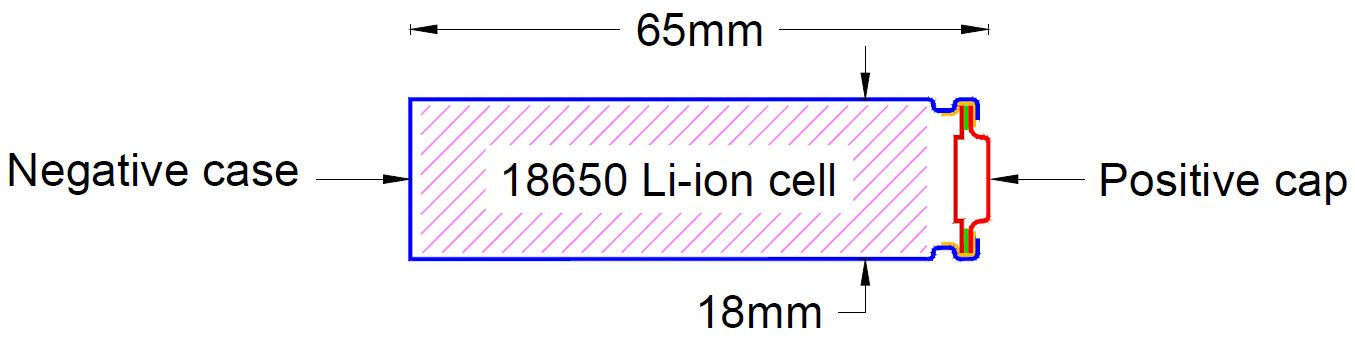
\includegraphics[width=0.5\paperwidth]{Images/image_5_1_(cell_diagram).png}
  \end{figure}

  \subsection{Where to find second hand 18650 lithium cells} % (fold)
  \label{sub:where_to_find_second_hand_18650_lithium_cells}

    For this guide, we will focus on recovering cells from laptop batteries. Old laptop batteries are regularly disposed of, so are waste items that are relatively easy to get hold of. Cordless power tool battery packs also have 18650 cells, but these may be a different chemistry to those found in laptop batteries, so check before using them. Newer batteries are more likely to have good cells - lithium-ion cells will self-discharge if left unused, so the cells in old batteries that haven’t been used for over a year are more likely to be discharged to the point where they can’t be recovered.

  % subsection where_to_find_second_hand_18650_lithium_cells (end)

  \subsection{18650 cell configurations} % (fold)
  \label{sub:18650_cell_configurations}

    A laptop battery pack will have inside it several 18650 lithium-ion cells connected together, along with a battery management system (BMS) circuit board. You can get a good idea of the number and configuration of cells inside a battery pack by checking the voltage and capacity. 

    A battery with a voltage of 10.8V or 11.1V will have three sets of cells in series (3 \(\times\) 3.6V or 3.7V), whereas a battery with a voltage of 14.4V or 14.8V will have four sets of cells in series (4 \(\times\) 3.6V or 3.7V)

    18650 lithium-ion cells will usually have a capacity of 2000-2400 milli-Amp-hours (mAh) per cell. Cells in series will have the same capacity as a single cell. If the laptop battery capacity is 2000-2400mAh, then there will be a single string of cells. A capacity of 4000-4800mAh indicates strings of two cells in parallel, and so on.

    If the battery capacity is shown in Watt-hours (Wh), you can calculate the capacity in mAh by dividing the Wh by the voltage and multiplying by 1000... e.g. 4000mAh = 1000 \(\times\) (44Wh \(\div\) 11.1V)

    % TODO INSERT IMAGE

    \begin{figure}[h!]
      \centering
      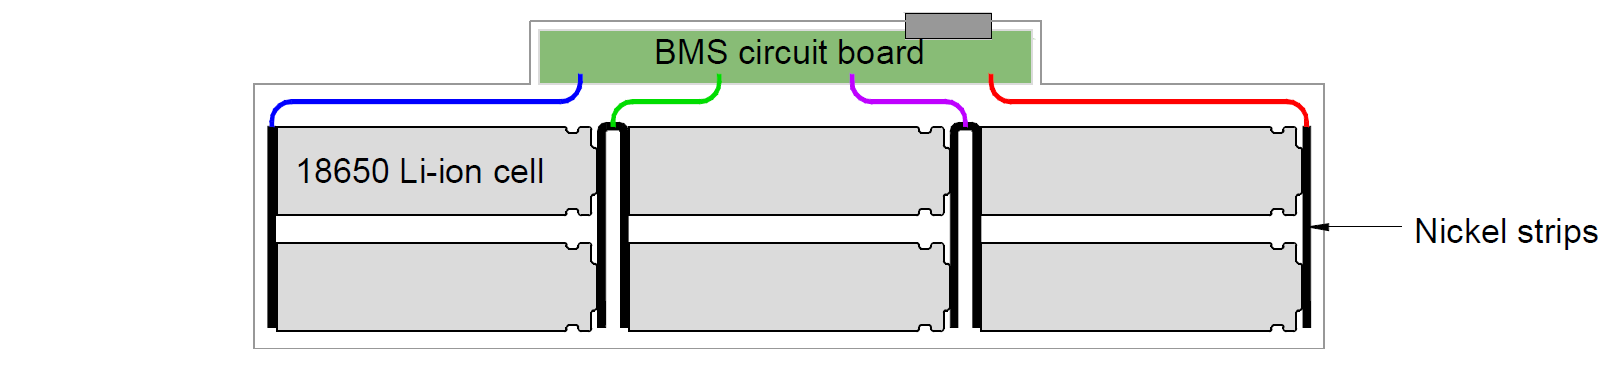
\includegraphics[width=0.75\paperwidth]{Images/image_5_2_(battery_configuration).png}
      \caption*{\centering Typical 6 cell laptop battery internal configuration}
    \end{figure}

    Because the cells that will be recovered are likely to have been used a lot, their actual capacity will be lower than that specified on the laptop battery. There is very little way of knowing how good the cells inside a laptop battery are without taking the battery apart, removing the cells, and testing them.
  
  % subsection 18650_cell_configurations (end)

  \subsection{How to safely recover 18650 lithium-ion cells from a laptop battery} % (fold)
  \label{sub:how_to_safely_recover_18650_lithium_ion_cells_from_a_laptop_battery}
  
    Risk warning - take extreme care not to short circuit lithium cells when removing them from laptop battery cases. 

    The first step is to open the plastic casing of the laptop battery. The best way to do this is to use a thin, flat blunt tool such as a flat-head screwdriver to prise the top and bottom of the case open, working along the seam from a weak point. You will need to take care not to injure yourself or damage the cells inside - it takes a bit of attention and practice to know the precise amount of force required. Some laptop batteries will be easier to open than others. Once you have enough separation between the top and bottom you can usually pull it open with your hands, although we recommend wearing some sturdy gloves for this.

    Once the case is opened, you can remove the lithium cells and the circuit board. You can then seperate cells into pairs or individual cells by cutting the nickel strips that connect the cells together. Before cutting any wires, identify the positive and negative sides of every cell - be sure to use any metal cutting tools on wires that won’t create a short circuit between any of the cells.

    \begin{figure}[!ht]
      \centering
      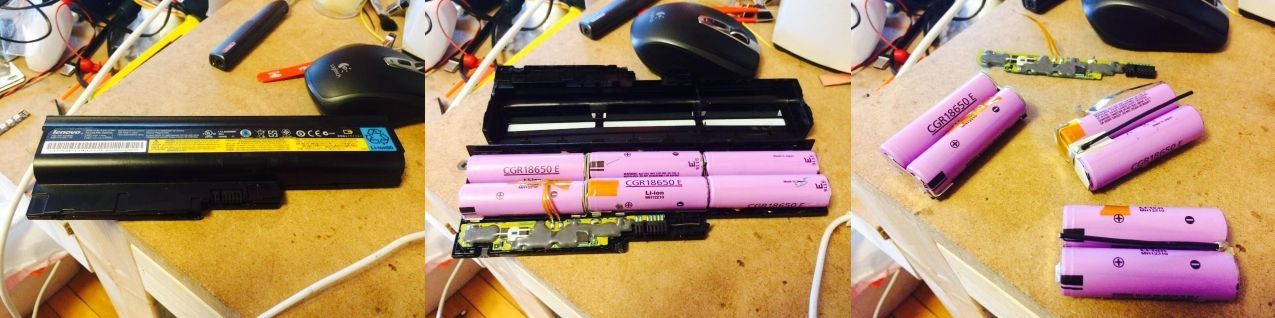
\includegraphics[width=0.75\paperwidth]{Images/image_5_3_(battery_disassembly).png}
    \end{figure}

    Any cells with damaged sleeves should be put to one side and disposed of safely or repaired with non-conductive electrical tape.

    Cells connected in pairs (or threes) should be kept together as much as possible, if they are to be used in a 2-cell or 4-cell USB power bank. Cut away the nickel strips connecting cells together, making sure to trim any sharp edges that might be left from where the nickel strip has been spot welded to the cell.

    Once the cells are separated and any excess tape, glue, etc is removed, you can attempt to identify them. You should be able to determine the brand (Panasonic, Samsung, LG and Sony are good brands to look for), and possibly their rated capacity. Since lithium-ion cells are not consumer items, they are unlikely to be labelled with much information about their technical specifications, but any identifying codes printed on the cells can be looked up online. Weigh the cells - good quality cells will weigh more than poorer cells. Their weight should be at least 40g.

    \begin{figure}[!ht]
      \centering
      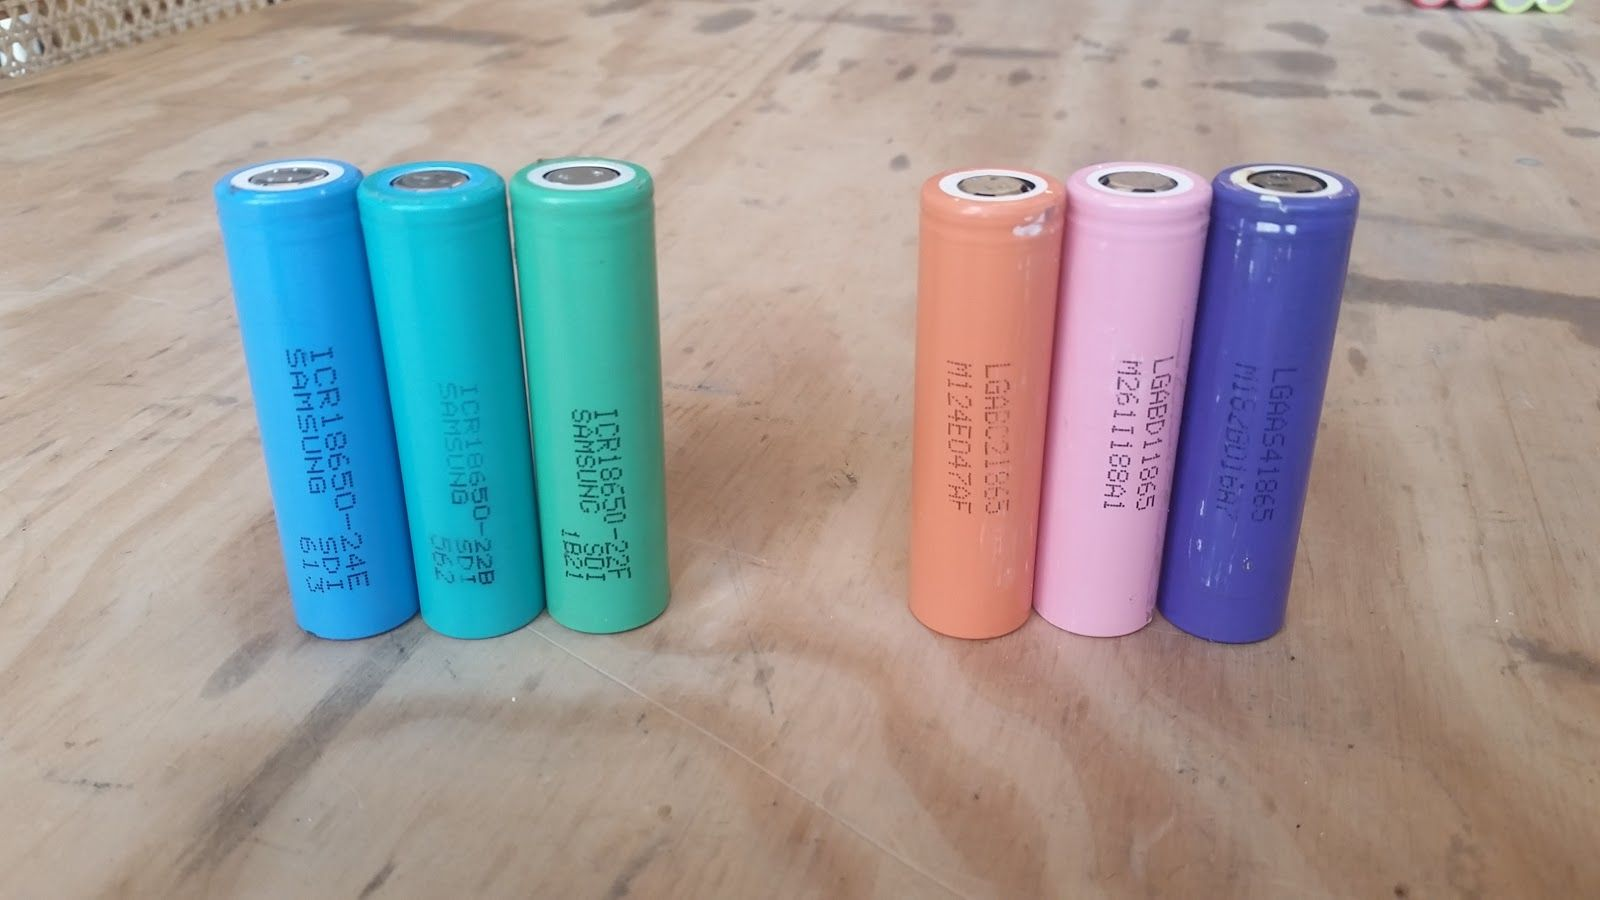
\includegraphics[width=0.4\paperwidth]{Images/image_5_4_(samsung_lg_cells).png}
      \caption*{\centering A selection of 18650 cells - Samsung on the left, and LG on the right}
    \end{figure}

  % subsection how_to_safely_recover_18650_lithium_ion_cells_from_a_laptop_battery (end)

  \subsection{How to test 18650 cells} % (fold)
  \label{sub:how_to_test_18650_cells}

    Risk warning - never use lithium-ion cells that have not been tested.

    You must test 18650 cells before you use them due to the risk of expired or defective cells catching fire. For small projects such as making USB power banks, where cells are only going to be connected in parallel with other cells, the testing is fairly simple, but for larger more complex projects you will need to test cells extensively before using them.

    The first thing to do is to measure the voltage of the cells as they come out of the battery packs. You will usually find that there will be at least one set of cells in each battery that will show a good voltage, and at least one set with a much lower voltage. This is due to how cells in series will become unbalanced over time, so there will always be one set of cells in every laptop battery that is working harder than the others, that will fail sooner.

    Cells with a voltage over 3V (or a little under 3V) are within their normal operating voltage, so should be good to use straight away. Cells with a voltage under 2V should not be used. Cells with a voltage between 2V and 3V will need to be charged with a lithium cell charger (e.g. a Nitecore i4) and then left for at least 24 hours to measure their ability to hold a charge before they can be used in a power bank.

    \begin{figure}[!ht]
      \centering
      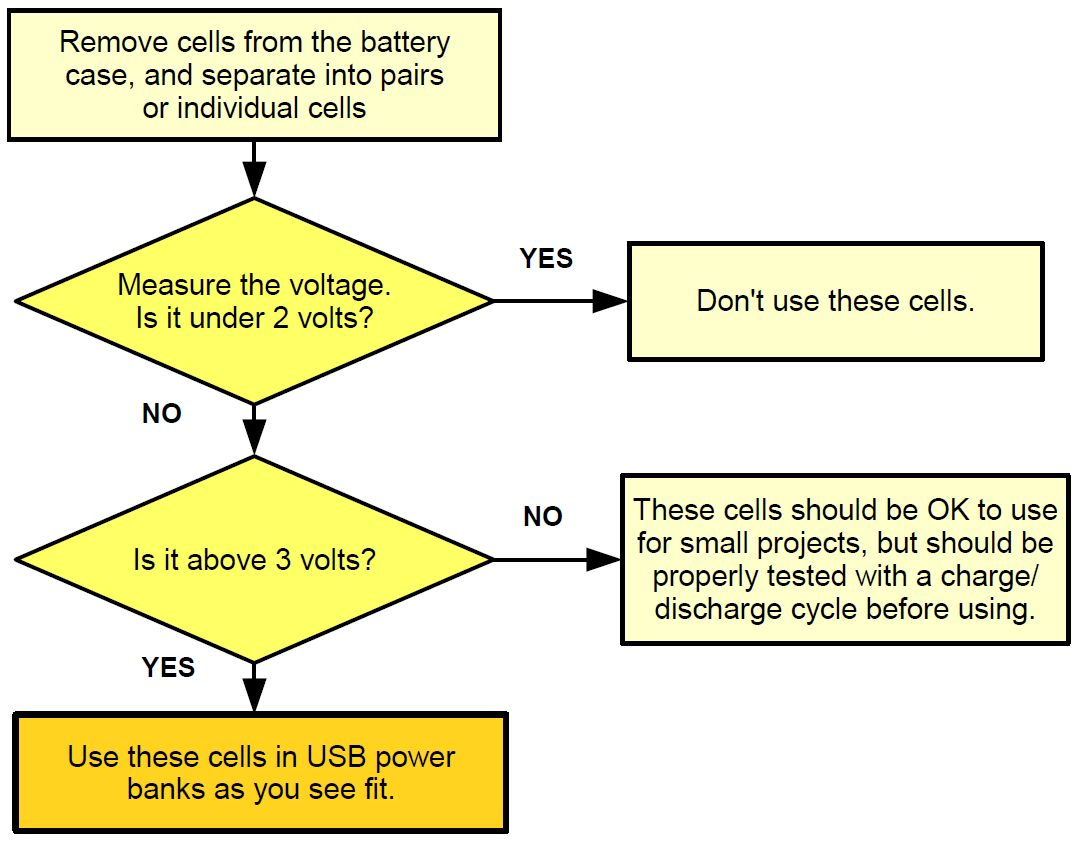
\includegraphics[width=0.75\paperwidth]{Images/image_5_5_(flowchart).png}
    \end{figure}

    To find out the actual capacity (in milli-Amp-hours, or mAh) of any used lithium cells, they will need to be put through a full charge-discharge cycle, to measure the capacity they provide on a full discharge. You can do this using a dedicated capacity tester (such as an iMax B6), or by putting the cells in a power bank and measuring the discharge capacity in mAh using a USB voltage tester or a USB load tester.
  
  % subsection how_to_test_18650_cells (end)

% section collecting_18650_cells_ (end)

\section{Building a USB power bank} % (fold)
\label{sec:building_a_usb_power_bank}

  USB power bank cases that will take 18650 cells without needing to do any soldering or complicated electrical work are fairly easy to find. These are good to use because once you have a collection of tested 18650 cells, you can simply slot them into the cases. Power bank case models that hold different quantities of cells are available - from single cell power banks up to 8 cell power banks. Adding more cells in parallel will increase the overall capacity of the power bank - an 8-cell power bank will store 8 times the energy of a single-cell power bank (assuming the cells are identical). Having multiple cells in parallel will mean that the load on each cell is shared evenly, so they should not become imbalanced the way cells in series will. Multiple cells in parallel will each be doing less work than a single cell for the same load, so they should last much longer. 

  While bigger power banks allow for more storage capacity, they will take up more space and weigh more, so you should consider how portable you need it to be, how much storage you would need from a power bank, and how often it will be used. Also, cases that have an indicator to show the battery charge level are much more useful than those that don’t. 

  \begin{figure}[!ht]
    \centering
    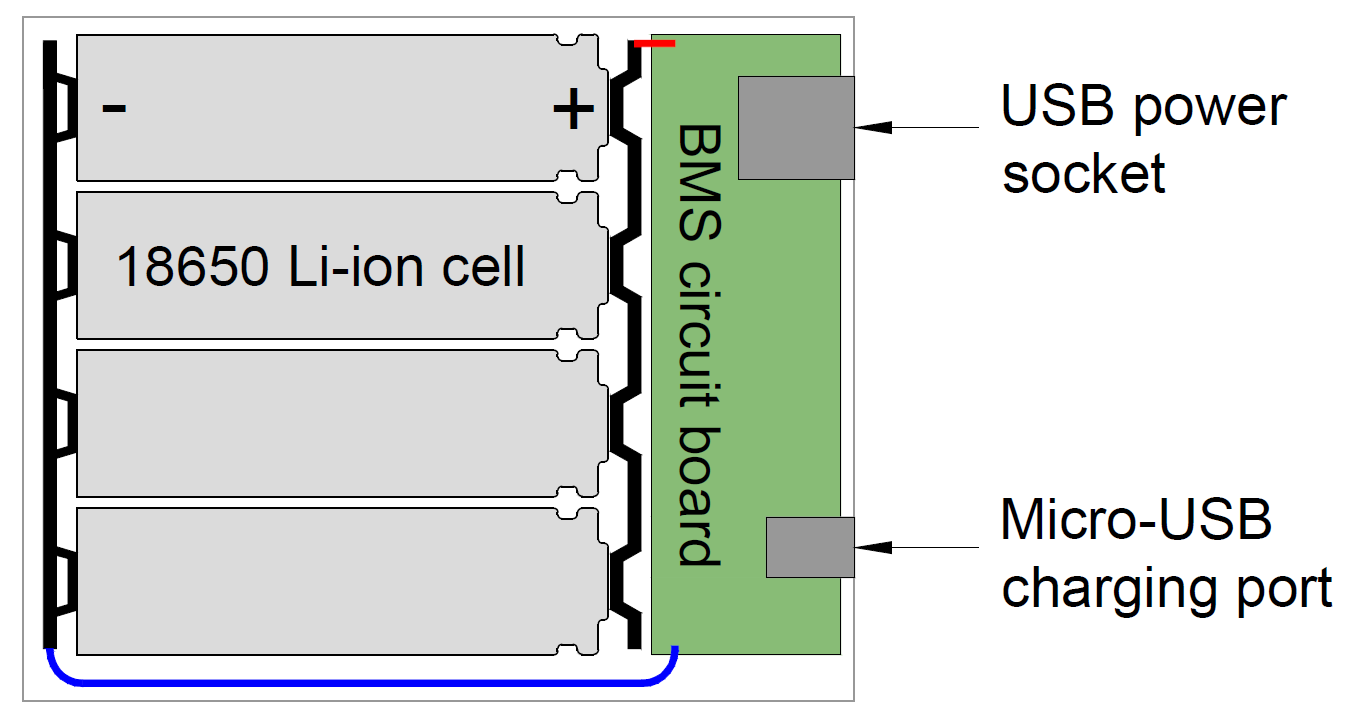
\includegraphics[width=0.35\paperwidth]{Images/image_6_1_(power_bank_diagram).png}
    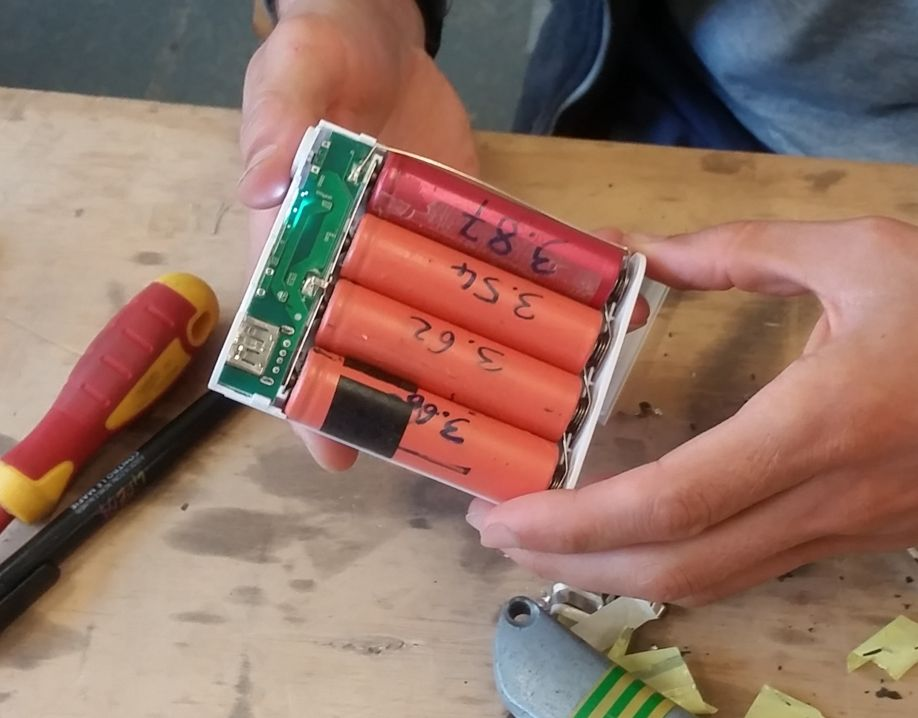
\includegraphics[width=0.30\paperwidth]{Images/image_6_2_(power_bank).png}
  \end{figure}

  Some cases require cells to be soldered together with metal strips along the positive and negative end of the cells. If cells have to be soldered, it is best to do it as quickly as possible to minimise damage to the cells. Use a large, powerful soldering iron that can provide much more thermal capacity - the more thermal capacity in your soldering iron, the less time it will take to solder each connection. Another option for connecting cells together is to spot-weld the connections onto the cells. Spot welding is the method that lithium battery manufacturers use, but it can be harder to DIY. 

  The circuit board in a USB power bank will include a battery management system that includes voltage converters to step the voltage from the battery up and down when it is providing power to or receiving power from a USB port (the standard voltage of a USB power supply is 5V). It also includes all the circuitry to manage the charge cycle of the battery.

  If you don’t want to buy a power bank case, or you aren’t able to get hold of one, you can always make your own. You will need to connect cells together, and then connect them to a USB charger circuit board, and a USB socket, and build an enclosure to contain them all. You can also include a switch to turn the power bank off when it is not being used. Building your own case allows for all kinds of customisation in the design, and the ability to add extra features that you can’t get in pre-built cases.

% section building_a_usb_power_bank (end)

\section{Building a bigger battery pack} % (fold)
\label{sec:building_a_bigger_battery_pack}

  A lithium battery pack to be used in higher voltage systems will need to be made up of several cells connected in series. Three lithium-ion cells with a nominal voltage of 3.7V connected in series will have an overall nominal voltage of 11.1V, and 12.6V when fully charged, so can feasibly be used in a 12V system. Seven lithium-ion cells in series will have a nominal voltage of 25.9V and a max voltage of 29.4V, which makes it a good option for 24V systems. It is essential to use a battery management system (BMS) that can keep the individual cells balanced, to avoid individual cells becoming overcharged or undercharged when they are subjected to charge-discharge cycles. It is also essential to ensure that the cells used have similar capacities, which will require a more thorough testing process if using used cells than that described above for making USB power banks. 

  While it is possible to build DIY battery packs to use in off grid systems from used 18650 cells connected in series, we do not recommend this unless you have a lot of experience of building off grid systems and working with these kind of cells, since the risks involved are considerable.

  If you are looking for lithium batteries to use in 12V renewable energy systems, we would recommend using pre-made lithium battery modules such as those made by TN Power or Victron, which are designed to be ‘drop-in’ replacements for 12V lead-acid batteries. These types of batteries tend to use lithium iron phosphate (LiFePO4) cells, which are much more thermally stable and safer to use than lithium-ion cells.

  You can find further information about how to design a basic off grid energy system in our \href{https://www.demandenergyequality.org/get-started-with-offgrid}{Intro to Off Grid guide}.

% section building_a_bigger_battery_pack (end)

\section{Lithium battery chemistries, applications and form factors} % (fold)
\label{sec:lithium_battery_chemistries_applications_and_form_factors}
  
  \textbf{Lithium Cobalt Oxide (LCO) -} a very common battery chemistry, used for batteries in phones and laptops and other small portable devices. They have a relatively short life span, low thermal stability and limited power capacity, but have a high energy density and are relatively cheap to make.

  \textbf{Nickel Manganese Cobalt (NMC) -} found in electric vehicles, grid-scale battery systems, e-bikes, power tools. They have a high power capacity, high energy density, and are more stable than LCO batteries.

  \textbf{Lithium Manganese Oxide -} mixed with NMC to further increase power capacity.

  \textbf{Lithium Iron Phosphate (LiFePO4) -} a very stable lithium chemistry mainly used in 12V battery replacements, cordless tools, and devices that need long lifespans. LiFePO4 cells have a lower nominal voltage and a lower energy density than other lithium chemistries, as well as being more expensive, but they are less susceptible to deterioration when fully charged, and are much safer. 

  The chemistry of lithium based cells applies to the cathode, with the anode being generally made of graphite (carbon). The cells are formed in multiple layers and sandwiched into a thin film, usually with an electrolyte-soaked porous separator in the centre and insulating separators on the outside. The film is either rolled into a cylinder and placed into a steel case, or folded and placed into a flat pouch (lithium polymer). Cylindrical cell sizes are designated by their diameter and length in mm, e.g 18-65(0). Lithium polymer (pouch) cells are used to create thin, flat batteries or lightweight batteries used to power drones and other RC vehicles.

% section lithium_battery_chemistries_applications_and_form_factors (end)

\section{Resources} % (fold)
\label{sec:resources}

  \subsection{Useful Information On Lithium Cells} % (fold)
  \label{sub:useful_information_on_lithium_cells}

    \begin{enumerate}
      \item How do lithium batteries work? \newline
        \url{https://batteryuniversity.com/learn/article/lithium_based_batteries}
      \item What’s inside an 18650 cell? And why it’s important: \newline
        \url{https://www.electricbike.com/inside-18650-cell/}
      \item 18650 things to do with an old laptop battery: \newline
        \url{https://www.wired.com/2011/09/18650-things-to-do-with-an-old-laptop-battery/}
      \item How to open laptop battery without damaging the cells: \newline
        \url{https://www.youtube.com/watch?v=7arwwTGliUA}
    \end{enumerate}
  
  % subsection useful_information_on_lithium_cells (end)

  \subsection{Other Renewable Energy Resources} % (fold)
  \label{sub:other_renewable_energy_resources}

    \begin{enumerate}[resume]
      \item Introduction to Off Grid Energy Systems: \newline
        \url{https://www.demandenergyequality.org/get-started-with-offgrid}
      \item DIY solar panels: \newline
        \url{https://www.demandenergyequality.org/build-your-own-panels}
      \item How solar cells work: \newline
        \url{https://www.demandenergyequality.org/guide-to-solar-energy}
      \item DIY bike power: \newline
        \url{https://www.demandenergyequality.org/build-your-own-bike-generators}
      \item DIY wind turbines: \newline
        V3 Power run courses: \url{http://v3power.co.uk/} \newline
        Hugh Piggott Designs: \url{http://scoraigwind.co.uk/}
      \item DIY micro hydro at Steward Wood Community: \newline
        \url{http://www.stewardwood.org/resources/hydroelectric.ghtml} \newline
        \url{https://www.permaculture.co.uk/articles/310505923/building-your-own-renewable-energy-systems-recycled-materials}
      \item Renewable energy diagram by Merlin Howse: \newline
        \url{http://offthegrid.org.uk/resources/renewable-energy-diagram-2.0.pdf}
    \end{enumerate}
  
  % subsection other_renewable_energy_resources (end)

  \subsection{Lithium battery suppliers for off grid systems} % (fold)
  \label{sub:lithium_battery_suppliers_for_off_grid_systems}

    \begin{enumerate}[resume]
      \item Wind and sun: \url{http://www.windandsun.co.uk/products/Batteries/Lithium-Ion-Batteries}
      \item Bimble solar: \url{https://www.bimblesolar.com/batteries/lithium-batteries}
    \end{enumerate}
  
  % subsection lithium_battery_suppliers_for_off_grid_systems (end)

% section resources (end)

\newpage

\appendix

\section{Equipment list} % (fold)
\label{sec:equipment_list}

  \subsection{Tools} % (fold)
  \label{sub:tools}

    \begin{itemize}
      \item Work gloves
      \item Eye protection
      \item Flat head screwdriver
      \item Wire cutters / side cutters
      \item Small-nose pliers
      \item Multimeter
      \item Marker pen for writing on cells
      \item Digital scales (optional)
      \item USB voltage tester (optional)
      \item Lithium cell charger, e.g. Nitecore Intellicharger (optional)
      \item Lithium cell charge-discharge capacity tester, e.g. iMax B6 (optional
    \end{itemize}
  
  % subsection tools (end)

  \subsection{Materials} % (fold)
  \label{sub:materials}

    \begin{itemize}
      \item Laptop battery (ideally last used less than a year ago)
      \item USB power bank case
      \item electrical tape
    \end{itemize}
  
  % subsection materials (end)

% section equipment_list (end)

\section{Using a multimeter} % (fold)
\label{sec:using_a_multimeter}

  \begin{figure}[!ht]
    \centering
    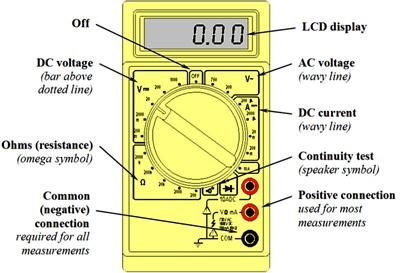
\includegraphics[width=0.65\paperwidth]{Images/image_a_1_(multimeter).png}
  \end{figure}

% section using_a_multimeter (end)

\end{document}